%------------------------------------------------------------------------------
%  report.tex
%------------------------------------------------------------------------------
%
%	BA6 - Database systems
%
%	Authors :
%		203267 - Bastien Antoine
%		183785 - Denoréaz Thomas
%		185078 - Dieulivol David
%
%	Versions :
%		2013.03.30 - Initial version
%

%--------------DOCUMENT--------------------------------------------------------
\documentclass[a4paper,oneside,11pt]{report}  % Type de document
\usepackage[english]{babel}

\usepackage{amsmath}
\usepackage{amsfonts}
\usepackage{amssymb}
\usepackage{mathspec}
\usepackage{fontspec}
\usepackage{xltxtra}
\usepackage{xunicode}
\usepackage[table]{xcolor}

%--------------PACKAGES--------------------------------------------------------
\usepackage[Bjornstrup]{fncychap}           % Chapitres
\usepackage{indentfirst}

\usepackage{fancyhdr}                       % Entete et pied de pages
\usepackage[outerbars]{changebar}           % Positionnement barre en marge externe
\usepackage[table]{xcolor}
\usepackage{lastpage}
%\usepackage{subfigure}
\usepackage{natbib}
\usepackage{paralist}
\usepackage{makeidx}                        % Permet de créer une indexation
\usepackage{multicol}                       % Gestion de plusieurs colonnes
\usepackage{multirow}
\usepackage{array}                          % 
\usepackage{a4wide}                         % Utilisation de toute la page A4
\usepackage[hmargin=2.5cm,vmargin=2.5cm]{geometry}

\usepackage{listings}                       % Affichage de code source

\usepackage{pifont}                         % Polices supplementaires
\usepackage{textcomp}
\usepackage{pgf}
\usepackage{tikz}
\usepackage{ae}                             % Affichage sous Adobe Reader
\usepackage{ifpdf}
\usepackage{url}
\usepackage{wrapfig}

\usepackage{graphicx}
\usepackage{caption}
\usepackage{subcaption}

\usepackage[disable]{todonotes}
%\usepackage{todonotes}

\usepackage{bytefield}

\usepackage{pgf}
\usepackage{tikz}
\usetikzlibrary{shapes}
\usetikzlibrary{arrows}
\usetikzlibrary{automata}

\DeclareTextCommandDefault{\nobreakspace}{\leavevmode\nobreak\ } 

%--------------PERSONNAL-INFORMATIONS------------------------------------------
\newcommand{\theversion}{1.0}

\newcommand{\myself}{Bastien Antoine, Denoréaz Thomas, Dieulivol David}
\newcommand{\titre}{Olympic Games}
\newcommand{\doctype}{Introduction to Database Systems}

%--------------MACROS----------------------------------------------------------
\newcommand{\nl}{\newline\indent}
\newcommand{\nol}{\newline\noindent}
\newcommand{\mathbox}[1]{\;\mbox{#1}\;}

%--- Elementary Algebra ---
\newcommand{\N}{\mathbb{N}}
\newcommand{\Nn}{\mathbb{N}^{*}}
\newcommand{\Z}{\mathbb{Z}}
\newcommand{\Zn}{\mathbb{Z}^{*}}
\newcommand{\Q}{\mathbb{Q}}
\newcommand{\R}{\mathbb{R}}
\newcommand{\Rp}{\mathbb{R}_{+}}
\newcommand{\Rm}{\mathbb{R}_{-}}
\newcommand{\Rn}{\mathbb{R}^{*}}
\newcommand{\Rpn}{\mathbb{R}_{+}^{*}}
\newcommand{\Rmn}{\mathbb{R}_{-}^{*}}
\newcommand{\C}{\mathbb{C}}

%\newcommand{\M}{\mathbb{M}}

\newcommand{\FF}{\mathcal{F}}
\newcommand{\GG}{\mathcal{G}}
\newcommand{\RR}{\mathcal{R}}
\newcommand{\PP}{\mathcal{P}}

\newcommand{\imp}{\Rightarrow}
\newcommand{\pmi}{\Leftarrow}
\newcommand{\equ}{\Leftrightarrow}
\newcommand{\Imp}{\;\Rightarrow\;}
\newcommand{\Pmi}{\;\Leftarrow\;}
\newcommand{\Equ}{\;\Leftrightarrow\;}

\newcommand{\nsubset}{\not\subset}
\newcommand{\ot}{\rightarrow}

\newcommand{\eqnpar}[1]{\left\{\begin{array}{lcl}#1\end{array}\right.}
\newcommand{\pareqn}[1]{\left.\begin{array}{lcl}#1\end{array}\right\}}

\newcommand{\appl}[5]{\begin{array}{llll}#1:&#2&\to&#3\\&#4&\mapsto&#5\end{array}}

\newcommand{\ddef}{D_{def}}

\newcommand{\liff}{\leftrightarrow}

%--- Geometry ---
\newcommand{\vect}[1]{\overrightarrow{#1}}
\newcommand{\coord}[1]{\left(\begin{array}{ccc}#1\end{array}\right)}

%--- Relational Algebra ---
\newcommand{\select}[2]{\left(\sigma_{#1}\ \entity{#2}\right)}
\newcommand{\project}[2]{\pi_{#1}\ \left(#2\right)}
\newcommand{\rename}[2]{\rho\left(\entity{#1},\ #2\right)}
\newcommand{\renamep}[3]{\rho\left(\entity{#1}\left(#2\right),\ #3\right)}
\newcommand{\join}{\;\bowtie\;}
\newcommand{\entity}[1]{\mbox{#1}}

% ----- LISTINGS ------------------------------------------------------------
\definecolor{ltgray}{rgb}{0.98,0.98,0.98}
\definecolor{ltbluegray}{rgb}{0.97,0.97,1}
\definecolor{dkred}{rgb}{.4,0,0}
\definecolor{ltred}{rgb}{.75,0,0}
\definecolor{dkgreen}{rgb}{0,0.5,0}
\definecolor{ltgreen}{rgb}{0,0.75,0}
\definecolor{dkblue}{rgb}{0,0,.4}
\definecolor{ltblue}{rgb}{0,0,.75}
\definecolor{dkcyan}{rgb}{0,0.4,0.4}
\definecolor{ltcyan}{rgb}{0,0.75,0.75}

\definecolor{nameclr}{rgb}{0,0.4,0.6}
\definecolor{ltnameclr}{rgb}{0.7,0.9,1}
\definecolor{dknameclr}{rgb}{0,0.2,0.3}
\newcommand{\namesty}[1]{{\color{nameclr}\textit{#1}}}

\lstset{
  language          = SQL,                  % langage par dfaut
  captionpos        = b,                    % position du caption
  numbers           = left,                 % affichage des numro de lignes
  frame             = trBL,                 % cadre du listing
  tabsize           = 3,                    % taille de la tabulation
  showtabs          = false,                % type de tabulation
  showspaces        = false,                % type d'espace
  showstringspaces  = false,                % type d'espace pour les chanes
  basicstyle        = \small\ttfamily,      % style du listing
  commentstyle      = \color{dkgreen}\itshape, % Comment Style
  stringstyle       = \color{ltred}\slshape, % Strings Style
  keywordstyle      = \color{nameclr}\textbf, % Keyword style
  breaklines        = true,                 % permet de sparer les lignes
  breakatwhitespace = true,                 % spare strictement aux espaces
  postbreak         = \Pisymbol{pzd}{229},  % symbol devant la coupure
  backgroundcolor   = \color{ltbluegray},
  linewidth         = \textwidth,
  xleftmargin       = 0.05\textwidth,
  xrightmargin      = 0.05\textwidth
}

% --- Macro pour les listings ---
\newcommand{\inputlisting}[1]
{\lstinputlisting[caption=#1]{dev/#1}}

% ----- PDF -----------------------------------------------------------------
\usepackage{graphicx, color}        % insertion images et couleurs
\graphicspath{{pic/}}
\DeclareGraphicsExtensions{.jpg,.png,.JPG}  % Formats d'images
\usepackage{pslatex}                        % Polices PDF, moins lourdes et non bitmap

\usepackage[                         %   Paramètrage de la navigation
    bookmarks         = true,               % Signets
    bookmarksnumbered = true,               % Signets numérotés
    pdfpagemode       = UseNone,            % Signets/vignettes fermé à l'ouverture
    pdfstartview      = FitR,               % La page prend toute la largeur
    pdfpagelayout     = OneColumn,          % Vue par page
    colorlinks        = false,              % Liens en couleur
    pdfborder         = {0 0 0}             % Style de bordure
    ]{hyperref}                             % Utilisation de HyperTeX

\usepackage{hypcap}
    
\hypersetup{                                % Information sur le document
    pdfauthor   = {\myself},
    pdftitle    = {\titre},
    pdfsubject  = {\doctype},
    plainpages  = false
}

\usepackage{pdfpages}                       % permet d'inclure des fichiers entiers pdf

%--------------ENTETE-ET-PIED-DE-PAGE------------------------------------------
\pagestyle{headings}

\pagestyle{fancy}
\renewcommand{\headrulewidth}{0.5pt}
\renewcommand{\footrulewidth}{0.5pt}

%\lhead{}
%\chead{}
%\rhead{}
\lfoot{\textcopyright EPFL - IC - Version \theversion}
\cfoot{}
\rfoot{\thepage\ on \pageref{LastPage}}

%--------------PAGE-DE-GARDE---------------------------------------------------

\title{{\huge \doctype}\\\vspace{1em}{\Huge \titre}\\\vspace{4em}
\includegraphics[width=0.5\textwidth]{logo_epfl}}
\author{Bastien Antoine (203267)\\ Denoréaz Thomas (183785)\\ Dieulivol David (185078)}
\date{Academic years 2012-2013\\\texttt{(\today)}}

\makeindex

\newcommand{\insertblankpage}{\newpage\thispagestyle{empty}\mbox{}\newpage}
\newcommand{\compref}[1]{\ref{#1} on page~\pageref{#1}}
\newcommand{\todoline}[1]{\todo[inline]{\textbf{TODO:} #1}}
\newcommand{\xxxline}[1]{\todo[inline]{\textbf{XXX:} #1}}
\newcommand{\fixmeline}[1]{\todo[inline]{\textbf{FIXME:} #1}}

\newcommand{\bitsbox}[3][lrt]{\bitbox[#1]{#2}{\raisebox{-3em}{#3}}}


%\newcommand{\descbox}[2]{\parbox[c][3.8\baselineskip]{0.95\width}{%
% facilitates the creation of memory maps. Start address at the bottom,
% end address at the top.
% syntax:
%   \memsection{end address}{start address}{height in lines}{text in box}
\newcommand{\memsection}[4]{%
  % define the height of the memsection
  \bytefieldsetup{bitheight=#3\baselineskip}%
  \bitbox[]{10}{%
    \texttt{#1}%      print end address
    \\
    %   do some spacing
    \vspace{#3\baselineskip}
    \vspace{-2\baselineskip}
    \vspace{-#3pt}
    \texttt{#2}%
  }%
  \bitbox{16}{#4}% 
}



% ----- DEBUT DU DOCUMENT ---------------------------------------------------
\begin{document}

% ----- Title + Logos -----

% --- Logo LAP + EPFL ---
%\begin{figure}[t]
%	\centering
%	\includegraphics[width=\textwidth]{header}
%	\subfigure{
%		\includegraphics[height=6em]{logo_lap}
%		\hspace*{\fill}
%		\raisebox{2.65em}{
%			\begin{tabular}{c}
%				\textsf{\textbf{\Large Processor Architecture Laboratory}}\\
%				\textsf{\textbf{\Large Laboratoire d'Architecture des Processeurs}}\\
%				\\
%				\textsf{School of Computer and Communication Sciences}
%			\end{tabular}
%		}
%		\hspace*{\fill}	
%		
\includegraphics[height=6em]{logo_epfl}
%	}
%\end{figure}

\begin{figure}[b]
	\centering
	
\includegraphics[height=6em]{logo_mysql}
	\hspace*{\fill}
	
\includegraphics[height=3em]{logo_play}
	\hspace*{\fill}	
	
\includegraphics[height=3em]{logo_scala}
\end{figure}

\newpage

\maketitle                                  % Titre du document

% ----- Quote -----

%\insertblankpage
\newpage

\thispagestyle{empty}
\vspace*{\fill}

\begin{center}
\parbox{0.73\textwidth}{
\large \emph{\textquotedblleft The most important motivation for the research work that resulted in the relational model was the objective of providing a sharp and clear boundary between the logical and physical aspects of database management.\textquotedblright }}
\parbox{0.65\textwidth}{\begin{flushright}---\hspace{0.5em} Edgar F. Codd, February 1982\end{flushright}}
\end{center}

\vspace*{\fill}

% ----- Contents + Preface -----
\pagenumbering{roman}                       % Numerotation romaine

\tableofcontents                            % Table des matieres
%\listoffigures                              % Liste des images
%\listoftables                               % Liste des tableaux
%\lstlistoflistings                          % Liste des listings
\newpage

% ----- Main Document -----
\pagenumbering{arabic}                      % Numerotation arabe
%------------------------------------------------------------------------------
%  introduction.tex
%------------------------------------------------------------------------------
%
%	BA6 - Database systems
%
%	Authors :
%		203267 - Bastien Antoine
%		183785 - Denoréaz Thomas
%		185078 - Dieulivol David
%
%	Versions :
%		2013.03.30 - Initial version
%

\chapter{Introduction}

Bla bla bla


%------------------------------------------------------------------------------
% END OF DOCUMENT
%------------------------------------------------------------------------------
%------------------------------------------------------------------------------
%  er-model.tex
%------------------------------------------------------------------------------
%
%	BA6 - Database systems
%
%	Authors :
%		203267 - Bastien Antoine
%		183785 - Denoréaz Thomas
%		185078 - Dieulivol David
%
%	Versions :
%		2013.03.30 - Initial version
%

\chapter{Entity–relationship model}

\begin{figure}[h!]
	\centering
	\fbox{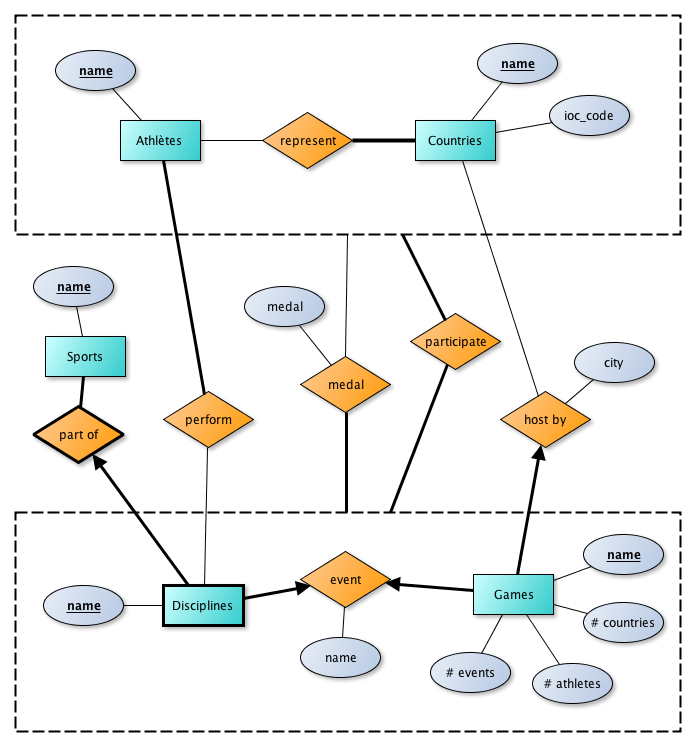
\includegraphics[width=0.5\textwidth]{er-model-old}}
	\caption{Previous ER Model.\label{fig:er-model-old}}
\end{figure}

From the analysis of the Dataset, here are our assumptions:

\begin{itemize}
	\item[$\circ$] An \textbf{Athlete} is always performing a \textbf{Discipline} instead of just a \textbf{Sport}.
	\item[$\circ$] An \textbf{Athlete} can represent only a \textbf{Country} for a \textbf{Game}. However, he can represent another \textbf{Country} for another \textbf{Game}.
	\item[$\circ$] A \textbf{Game} can only be hosted by one and only one \textbf{Country}, but this \textbf{Country} can host several \textbf{Games}.
	\item[$\circ$] Each \textbf{Discipline} is defined by its \textbf{Sport}.
	\item[$\circ$] An \textit{Event} is characterized by only a \textbf{Game} and only a \textbf{Discipline}.
	\item[$\circ$] A \textit{Medal} is obtained for a \textit{Representant} during an \textit{Event}.
	\item[$\circ$] A \textit{Participant} is formed by both a \textit{Representant} and an \textit{Event}.
\end{itemize}

\section*{Changes since deliverable 1}
After the first deliverable, we have made some simplifications to our model.
There are still two aggregations standing for a representative (\textbf{athlete} and \textbf{country}) and an event (\textbf{discipline} and \textbf{games}). These aggregations are bonded by the relation \textit{Representant\_participates\_Event} which models the participation from a representative to a \textbf{discipline}.
We have removed the other relations between them because there is only redundant information and we can put the medal attribute in the participation relation.

\begin{figure}[h!]
	\centering
	\fbox{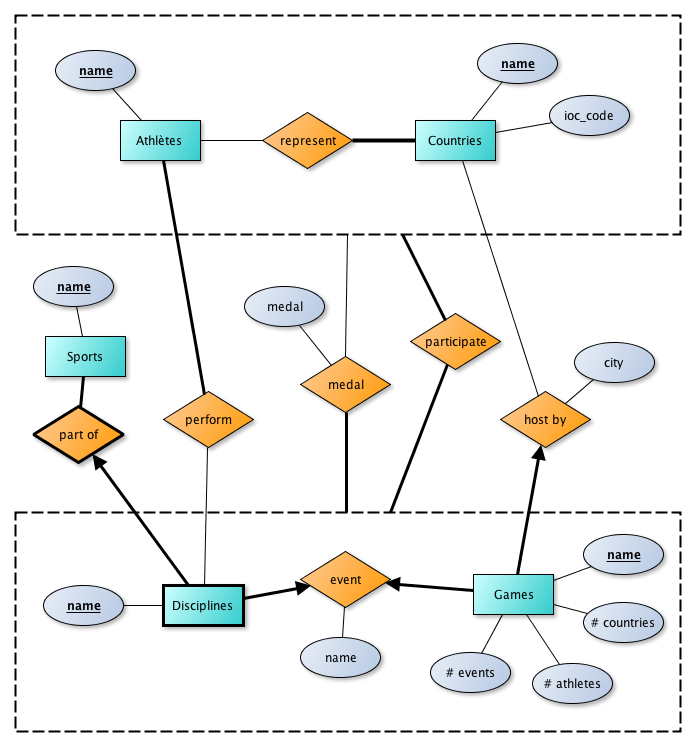
\includegraphics[width=0.8\textwidth]{er-model}}
	\caption{New ER Model.\label{fig:er-model}}
\end{figure}


%------------------------------------------------------------------------------
% END OF DOCUMENT
%------------------------------------------------------------------------------
%------------------------------------------------------------------------------
%  relational-schema.tex
%------------------------------------------------------------------------------
%
%	BA6 - Database systems
%
%	Authors :
%		203267 - Bastien Antoine
%		183785 - Denoréaz Thomas
%		185078 - Dieulivol David
%
%	Versions :
%		2013.03.30 - Initial version
%

\chapter{Relational schema and constraints}

Bla bla bla

\begin{center}
\lstinputlisting[caption={Salut}]{sql/example.sql}
\end{center}


%------------------------------------------------------------------------------
% END OF DOCUMENT
%------------------------------------------------------------------------------
%------------------------------------------------------------------------------
%  ddl-statements.tex
%------------------------------------------------------------------------------
%
%	BA6 - Database systems
%
%	Authors :
%		203267 - Bastien Antoine
%		183785 - Denoréaz Thomas
%		185078 - Dieulivol David
%
%	Versions :
%		2013.03.30 - Initial version
%

\chapter{Relational schema and constraints}

\section{Relational schema}

\begin{figure}[h!]
	\centering
	\fbox{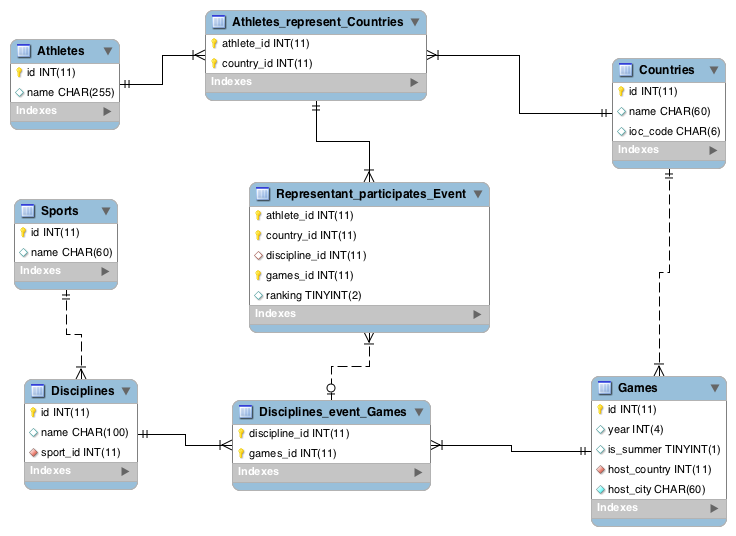
\includegraphics[width=0.9\textwidth]{ddl-scheme-new}}
	\caption{Generated EER Model from MySQL Workbench.\label{fig:ddl-scheme}}
\end{figure}
After implementing the DDL from Section \ref{sec:ddl}, we generated the scheme in Figure \ref{fig:ddl-scheme} using MySQL Workbench.

\newpage
\section{SQL Data definition language statements}
\label{sec:ddl}

We decided to implement our project, using the Oracle MySQL database management system. Following is the listing of our entities and relations.

We changed the DDL adding the unique constraints because we had to much duplicate during the import.

\begin{center}
	\lstinputlisting[caption={DDL Entities}]{scripts/ddl-entities.sql}
\end{center}
\newpage

\begin{center}
	\lstinputlisting[caption={DDL Relations}]{scripts/ddl-relations.sql}
\end{center}


%------------------------------------------------------------------------------
% END OF DOCUMENT
%------------------------------------------------------------------------------

% ----- Appendices -----
%\appendix
%\part*{Appendix}
%\addcontentsline{toc}{part}{Appendix}

%\input{tex/appendixA}

% ----- References -----
%\newpage
%\normalsize
%\nocite{*}
%\renewcommand{\bibname}{References}
%\bibliographystyle{unsrtnat}
%\begin{small}
%\bibliography{bib/bibliographie}
%\end{small}

% ----- Index -----
%\newpage
%\addcontentsline{toc}{chapter}{Index}
%\printindex

% ----- Index -----
\newpage
\addcontentsline{toc}{chapter}{Todo}
\listoftodos

\end{document}

% ----------------------------------------------------------------------------
% ----- END OF DOCUMENT ------------------------------------------------------
% ----------------------------------------------------------------------------